\documentclass[pdftex,12pt,a4paper]{article}
\usepackage[pdftex]{graphicx}
\usepackage{listings}
\usepackage{color}
\usepackage{graphicx}

\newcommand{\HRule}{\rule{\linewidth}{0.5mm}}	%title.tex
\newcommand{\code}[1]{\texttt{#1}}

\definecolor{mygreen}{rgb}{0,0.6,0}
\definecolor{mygray}{rgb}{0.5,0.5,0.5}
\definecolor{mymauve}{rgb}{0.58,0,0.82}

\lstset{ %
  backgroundcolor=\color{white},   % choose the background color; you must add \usepackage{color} or \usepackage{xcolor}
  basicstyle=\footnotesize,        % the size of the fonts that are used for the code
  breakatwhitespace=false,         % sets if automatic breaks should only happen at whitespace
  breaklines=true,                 % sets automatic line breaking
  captionpos=b,                    % sets the caption-position to bottom
  commentstyle=\color{mygreen},    % comment style
  deletekeywords={...},            % if you want to delete keywords from the given language
  escapeinside={\%*}{*)},          % if you want to add LaTeX within your code
  extendedchars=true,              % lets you use non-ASCII characters; for 8-bits encodings only, does not work with UTF-8
  frame=single,                    % adds a frame around the code
  keepspaces=true,                 % keeps spaces in text, useful for keeping indentation of code (possibly needs columns=flexible)
  keywordstyle=\color{blue},       % keyword style
  language=Octave,                 % the language of the code
  morekeywords={*,...},            % if you want to add more keywords to the set
  numbers=none,                    % where to put the line-numbers; possible values are (none, left, right)
  numbersep=5pt,                   % how far the line-numbers are from the code
  numberstyle=\tiny\color{white}, % the style that is used for the line-numbers
  rulecolor=\color{white},         % if not set, the frame-color may be changed on line-breaks within not-black text (e.g. comments (green here))
  showspaces=false,                % show spaces everywhere adding particular underscores; it overrides 'showstringspaces'
  showstringspaces=false,          % underline spaces within strings only
  showtabs=false,                  % show tabs within strings adding particular underscores
  stepnumber=2,                    % the step between two line-numbers. If it's 1, each line will be numbered
  stringstyle=\color{mymauve},     % string literal style
  tabsize=2                       % sets default tabsize to 2 spaces
}

\begin{document}
	\begin{titlepage}

\begin{center}

\textsc{\LARGE CS12130 Individual programming project}\\[1.5cm]


\HRule \\[1.5cm]

\emph{Author:}\\
Nicholas Dart\\
\emph{nid21@aber.ac.uk\\130057750}

\vfill

% Bottom of the page
{\large \today}

\end{center}


\end{titlepage}
	\tableofcontents
	\newpage
	\pagestyle{plain}

	\section{Self Evaluation}
	\emph{Year:} 2013 - 2014
	\emph{Module:}     CS12130\\
	\emph{Assignment Number:}         1\\
	\emph{Assignment Description:}   Individual Programming Project\\
	\emph{Worth} 30\% \emph{of final mark for this module}\\
	\emph{How many hours (approx.) did you spend on this assignment?} 60\\
	\emph{Expected Letter Grade:} B (65\%)\\
	\emph{And why?}\\
	Programmatically all the elements of the specification are there, the four versions of the player, the region, the disease spreading, and have all been implemented in a way I feel is suitable and easy to read. I feel I've separated the basic components of the design into their separate classes sufficiently to allow future adjustment or complete overall of individual sections. I have tried not to use magic numbers, but instead use constants which are appropriately names, so that in the future the game can be more easily understood and modified 
	\\\emph{What did you Learn?}\\
	Polymorphism of a class. An abstract Player class allows for a single doLevel() function, whilst allowing it to take in any player, which may or may not do things like try to cure the disease, change region cells around it etc. I also learned of the benefits of doing class diagrams before a project, It helped to create a clear definition of which class is doing what, and where responsibility for actions lies. 
	\section{Overview and Requirements}
		The project must implement the so-called \emph{Spread and Die} game, it's requirements are as follows:
		\begin{itemize}
			\item There is a region or field of 12 by 12, each cell in the region represents a cell like a chest board, but contains one of between 2 and 4 (inclusively) region characters.
			\item There is a disease on the board, to start with a single cell is selected by the user to be the diseased cell. The disease can then spread from there.
			\item The disease spreads with each iteration or generation of the game. If the disease occupies a cell of a given region type, adjacent cells of the same region type become diseased with the next iteration, but other region types not of the same as the one the diseased cell occupies become infected first, and then diseased. 
			\item There are several levels of the game, one through to four, each with varying levels of difficulty for the player
			\item There is a player on the board, the player is placed randomly on the board, and depending on the level, it may try to do several things:
			\begin{enumerate}
				\item Level one has the player move randomly around the board, with no intelligent decision making or disease avoidance.
				\item Level two has the player try to avoid the disease, They may look at adjacent cells or look over the whole grid. They have no line of sight limit.
				\item Level three has the player try to avoid the disease as with player two, but also allows the player to alter cells directly adjacent in the region, this can either be done strategically or randomly.
				\item Level four has the player try to cure the disease, through what ever medium or way seems fit. The disease can be cured, but can also mutate, thus meaning that if a player is immune to the disease, they can stand on a diseased or infected cell, but only until it mutates. The player also moves as intelligently as in level two.
			\end{enumerate}
			\item The disease should be represented by a `D', infected cells by `I', the player by `P' and then up to four other symbols for the region characters.
			\item Each successful iteration of the game is counted as a point towards the player, at each level of the game, the player is required to get 20 points to pass to the next level of the game.
		\end{itemize}

		\subsection{Alterations from official specification}
		Some of the above listed requirements were interpretations of, or modifications to, the official specification for this project.
		\begin{itemize}
			\item It was not specified if the player or disease can move/spread diagonally or only to directly adjacent cells, I chose the latter as it decreases the speed of the disease and gives the Level one player more of a chance to succeed and pass to level two.
			\item It was not specified when the game should end, except in the event that the player is diseased, so I decided that the game should continue until such time, even if the score has reached that which is required to pass.
			\item It was not specified if the disease mutates as a whole, or on a cell by cell basis. I decided on the former because there is no easy way to represent to the user which individual cells are still a threat to the player and which are not. It was also not clear if the player, having once cured the disease, had won the game, respective of the generation count, or if the disease could then mutate and then infect the player again. The latter was chosen here as I feel it was a more interesting game mechanic and allows for longer game.
		\end{itemize}
	\section{Design and UML Diagrams}
		\subsection{Justification of Design}
		The obvious starting point for the project was to split the `Field' and `Player' elements from each other, as they interact with each other, but do not play a part of each others major functionality. The `player' will require some information from the `Field', such as the region types and infected state of cells on the board. Similarly the `Field' will need an update from the player as to where it wants to move to, and may respond if it's a valid move it not.

		This initial approach yielded two obvious starting classes, the `Player' and the `Field' (as well as a `Main' or starting class, which I am calling `RunGame' whose sole purpose is to provide an interface to the user, start the game and provide a joining point to the `Field' and `Player' classes). As I plan to include all four levels of the game, It was then logical to crate a class for each. I later refined my design to use an abstract to enforce the necessary functions, and extend the player from the abstract player class.
		\subsubsection{Initial UML Diagram}
			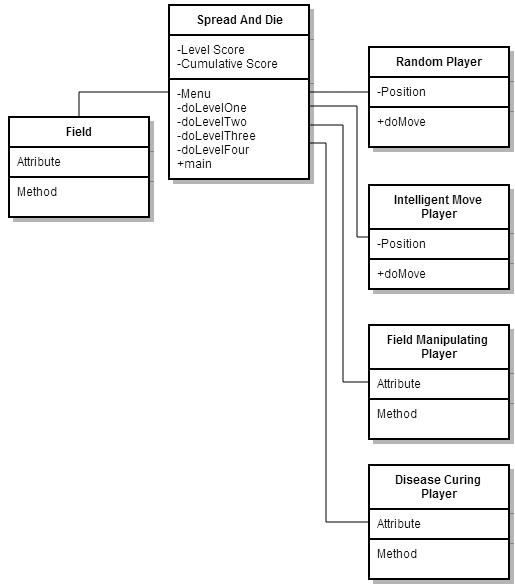
\includegraphics[width=\linewidth]{./fig1.png}
		\subsubsection{Final UML diagram}
			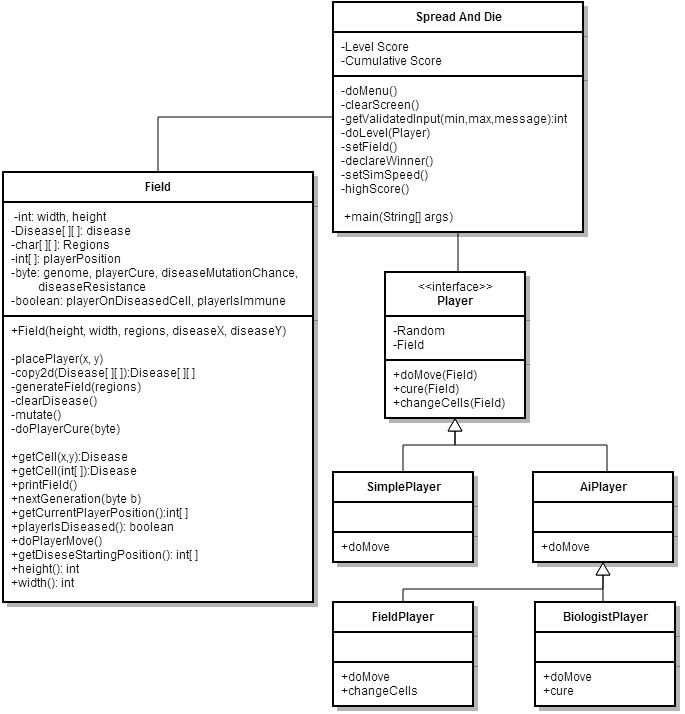
\includegraphics[width=\linewidth]{./fig2.png}
		\subsection{Class Descriptions}
			\subsubsection{RunGame Class}
			This class is largely the binding between the Player(s) and the Field, it gets the settings for the game, such as height and width of the field, simulation time, which player to use or if it should go through until all levels have been passed. It also contains the loop which will continue until the Field reports the payer is dead.
			\subsubsection{Field Class}
			The Field class contains the region cells, diseased/infected cells, player position and the cure/mutation of the disease as a whole. It also takes the players move, cure attempts and region adjustments and validates them. It is the class which simulates the next generation, taking into account the previously mentioned decisions from the player.
	\section{Running the Game}
		To compile the game, first cd to the game directory, then compile using \emph{javac}

		\$ javac RunGame.java
		\\To run the game, run \emph{RunGame} with \emph{java}

		\$ java RunGame\\
		\\The game has been implemented primevally in Linux, all major features work in Windows too, but for the optimal experience, a UNIX based system is advised. Note the only major advantage is the screen clearing.

		The main interface will allow you to:
		\begin{description}
			\item[0] Run the game in it's entirety, from level one through to level four
			\item[1] Run the game at level one only
			\item[2] Run the game at level two only
			\item[3] Run the game at level three only
			\item[4] Run the game at level four only
			\item[5] View the high score
			\item[6] Set the simulation speed, Note that higher values are larger waits between iterations. This value takes floating point numbers
			\item[7] Set the field width and height for all future fields generated
			\item[8] Quit the game nicely
		\end{description}

	\section{Autogenerated Javadocs}
		Javadocs generated from comments in the classes for public methods are available in the docs directory (see index.html), To update/recreate them use \emph{javadoc}

		\$ javadoc *.java -d docs
	\section{Further Design}
		\subsection{User Case Diagram}
			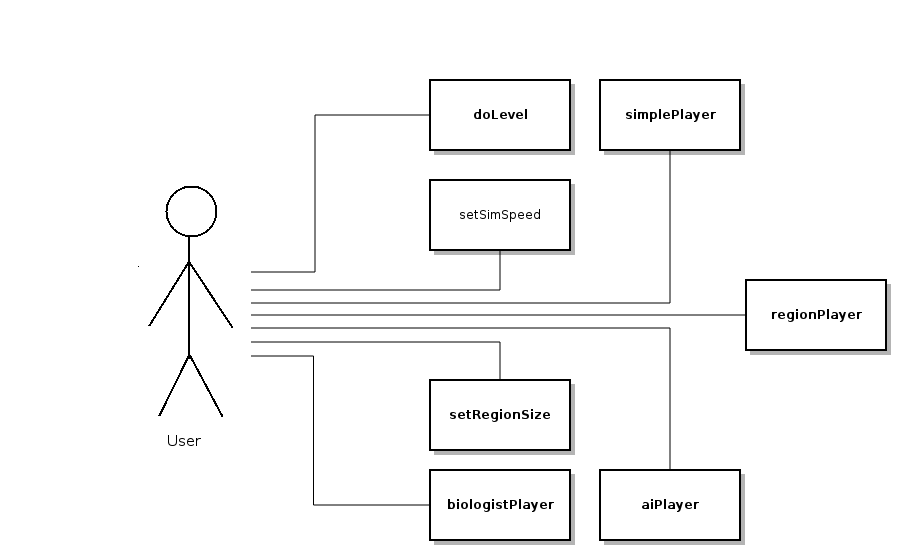
\includegraphics[width=\linewidth]{./fig3.png}
		\subsection{State Diagram}
			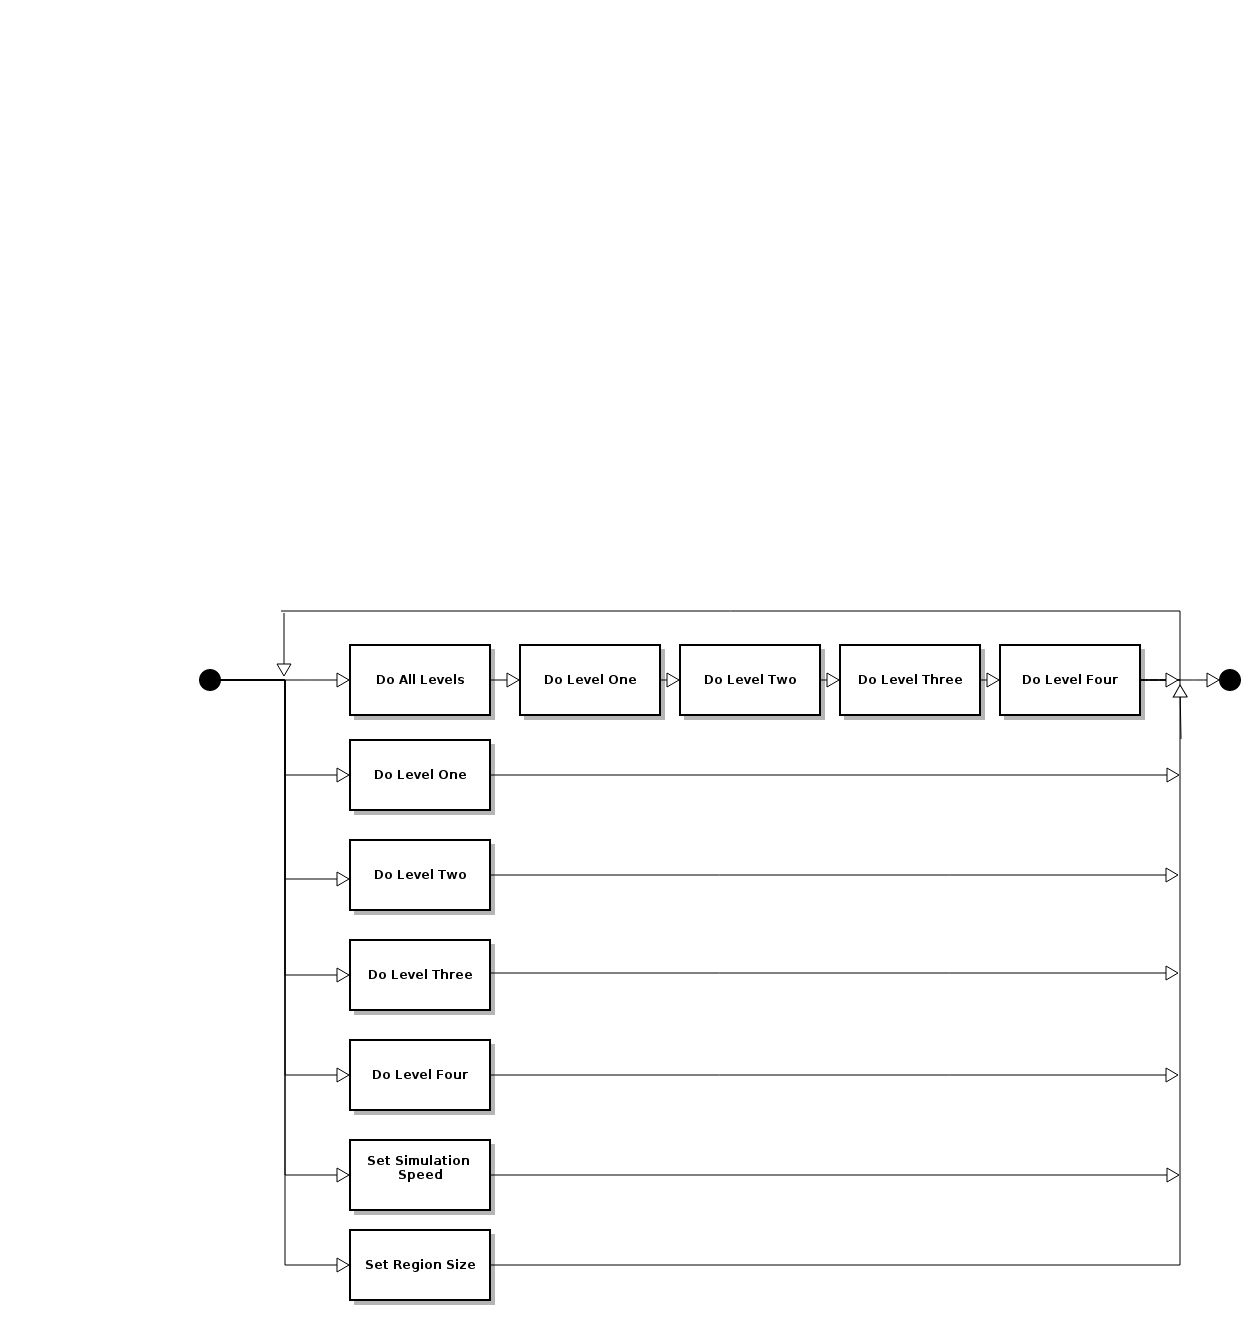
\includegraphics[width=\linewidth]{./fig4.png}
	\section{Testing and Later Design Decisions}
		Testing was largely done after completion of some basic functionality of the Field class; to test many other parts of the code, such as the player, I would have to implement something of equal functionality to the field, since the player requires the field for it's movement decisions.
		\subsection{Testing the Field}
			The Field class was implemented very slowly with much testing during it's development, as it is the most crucial and most depended class in the game. The first feature to be tested was the regions and disease arrays, which originally used chars instead of enums, checking that I was writing to them correctly, generating a random spread of region characters and that the two arrays would map/overlay together correctly. Once this was tested successfully, I moved on to testing the disease spreading, I know from experience that Java used shallow copying of it's objects and non-primitives, so I preemptively created and tested the copy2d method to give an exact copy of a 2d array instead of just crating a reference to it. I also know from experience that when dealing with games that iterate turn by turn, to simulate the next generation, one has to operate on a strict read only from the current generation array, and write to a (hard) copy of that array, otherwise multiple moves/spreads would be made in a single game tick. I next tested this by using a region with one region character, if the \emph{current} and \emph{next} generation arrays were references to one or the other, then I would expect the disease to spread multiple cells in a single iteration:  \\
			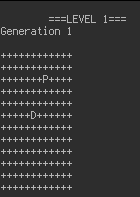
\includegraphics{./fig5.png}
			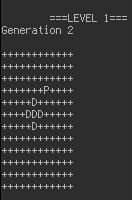
\includegraphics{./fig6.png}\\
			As can be seen in the above two images, the disease spreads only one cell in either direction as is required, I then continued the testing for two and then four region characters, both of which seem to work fine. I then moved on to work on the player movement validation, I had initially planed to have the player position within the player class it's self, but as I was going to have four different players, each of which would have to check that where it wants to move to is valid, I realized that having the player movement in the field would eliminate duplicate code. This was simply tested by placing the player on the edge of the field and trying to validate a move off the field, which the validation didn't allow, so would ask for another movement from the player. Ultimately this movement validation would be used most with the \emph{SimplePlayer} as it was random movements and so could try to move off the field.
		\subsection{Testing the SimplePlayer}
			This class was very simple, all it had to do as return a \emph{Field.Movement} enum in the direction it wanted to move, which being random, was a simple case of a for loop. Later when I worked on the BiologistPlayer and FieldPlayer, I included two more functions into the abstract Player class, these for the player simply returned either a byte of value 0 for the cure, or an empty Dictionary for the FieldManipulations.
		\subsection{Testing the AiPlayer}
			This required me to allow a lot more information to be accessible to the player, such as where the disease was originally placed and the cells around it. As these were mainly getters for values, I did not test these, but rather Checked the decision process of the player, the logic behind it was rather simple; the player should avoid the disease if it is near by, otherwise it should try to run to the corner furthest away, failing that a corner (as they will be the furthest points from the disease). This works fine most of the time, but on the occasion where the disease lies between the player and the furthest corner from the disease, the player would try running to the disease, only to run away again. I thought about using A* path finding to solve this, but on a standard 12x12 sized grid, the player didn't have enough time to run around the disease before it was boxed in, so I abandoned this in favor of the `Get to the nearest corner and stay there' approach. This was tested simply by printing which directions the player thought it could move, and then which one it was going to move it.
		\subsection{Testing the FieldPlayer}
			The FieldPlayer was tested by first attempting to construct a \emph{HashMap} of all the cells the player is trying to edit, and then the value that the player is trying to adjust them to, such that the position of the cell is the key and the new region type the value. Once this was checked, it was then a simple matter of adjusting the appropriate referenced cell in the field to the given value. 
		\subsection{Testing the BiologistPlayer}
			This player presented many further additions to the Field class, I chose a byte to represent the disease's genome or DNA, and then another byte to represent the players cure, if the cure is sufficiently close to the DNA of the disease, it is assumed the disease is cured, but if the disease then mutates sufficiently from it's current DNA, it is then considered to have mutated and the cure is now ineffective. I chose bytes because it has a small number of possibilities (256). During testing I found that it's range was from -128 to 127, which promoted a re-write of the logic I used to determine mutation and curing. Originally this player was a separate class, but when I realized that the only difference between the levels was really what the player tries to do, I adapted the players to inherit from an abstract player class, which I could then pass to the \emph{doLevel()} function in \emph{RunGame}. 
	\newpage
	\section{Examples of Expected Output}
		Setup for a 50x50 game\\
		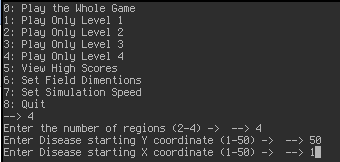
\includegraphics{./fig7.png}\\
		The 50x50 game\\
		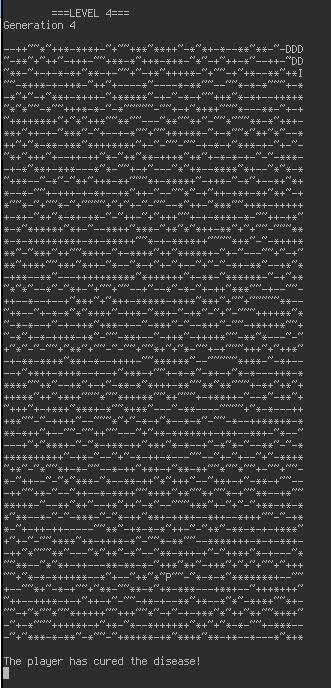
\includegraphics{./fig8.png}
	\section{Acknowledgments}
		\begin{itemize}
			\item Any references or help used in the creation of any functions or classes has been referenced where it is used within the code
			\item My peers helped spot minor bugs and/or logical errors
		\end{itemize}
	\section{Source Code}
		\subsection{RunGame.java}
			\lstinputlisting[language=Java]{RunGame.java}
		\subsection{Field.java}
			\lstinputlisting[language=Java]{Field.java}
		\subsection{Player.java}
			\lstinputlisting[language=Java]{Player.java}
		\subsection{SimplePlayer.java}
			\lstinputlisting[language=Java]{SimplePlayer.java}
		\subsection{RegionsPlayer.java}
			\lstinputlisting[language=Java]{RegionsPlayer.java}
		\subsection{AiPlayer.java}
			\lstinputlisting[language=Java]{AiPlayer.java}
		\subsection{BiologistPlayer.java}
			\lstinputlisting[language=Java]{BiologistPlayer.java}

\end{document}